\chapter{Oracle APEX Online}

\section{Langkah-langkah}
\begin{enumerate}
    \item Membuka aplikasi apex online, dan mengklik request a workspace
\begin{figure}[!htbp]
    \centering
    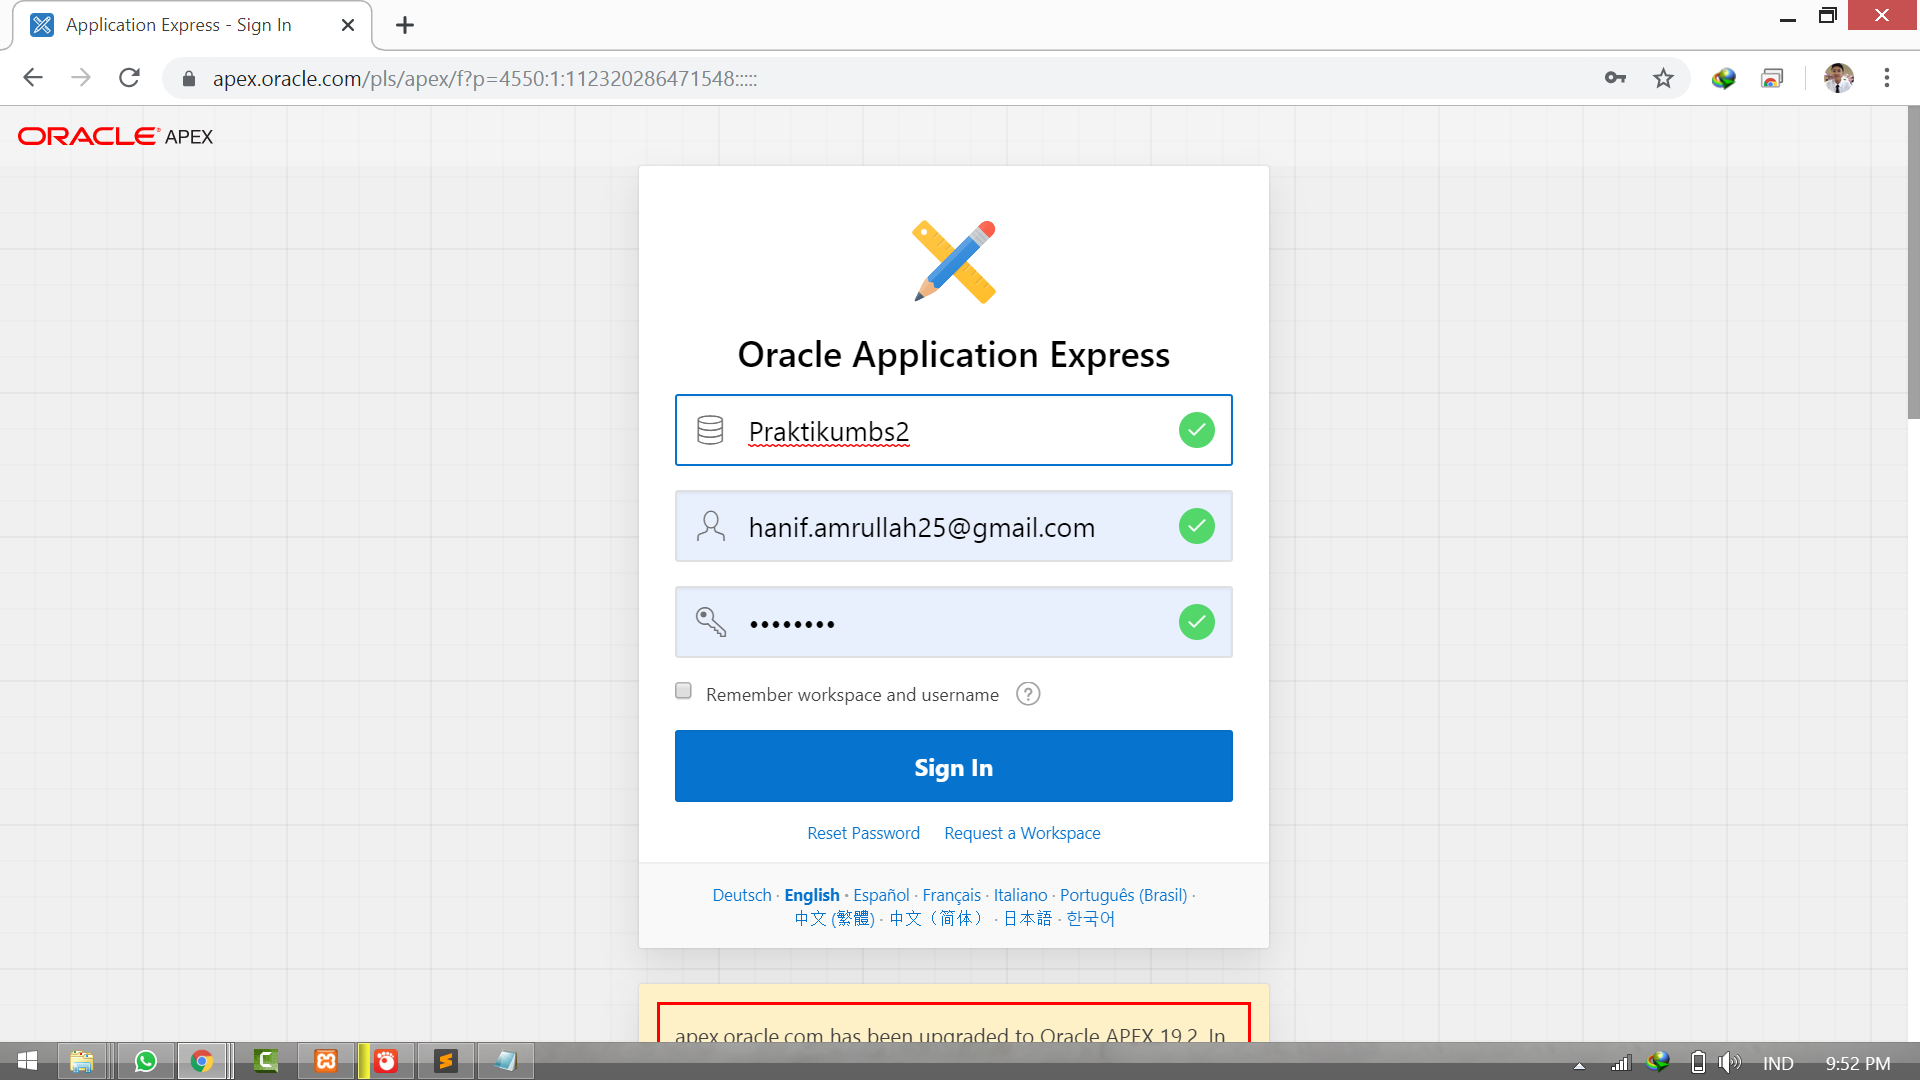
\includegraphics[scale=0.5]{section/gambar_bab1/1.JPG}
    \label{penanda}
\end{figure}
    \item membuat request a workspace
\begin{figure}[!htbp]
    \centering
    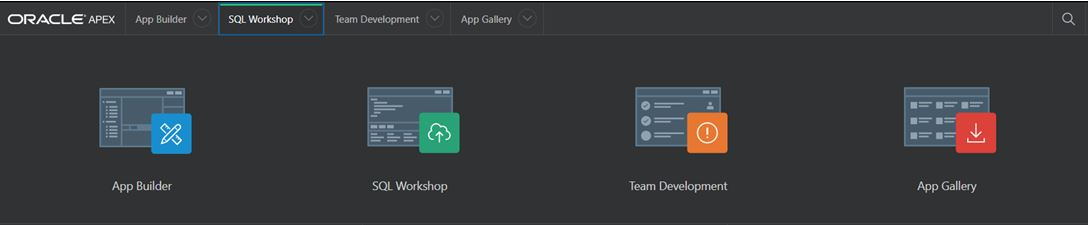
\includegraphics[scale=0.5]{section/gambar_bab1/2.JPG}
    \label{penanda}
\end{figure}
\begin{enumerate}
    \item Lalu klik next
\begin{figure}[!htbp]
    \centering
    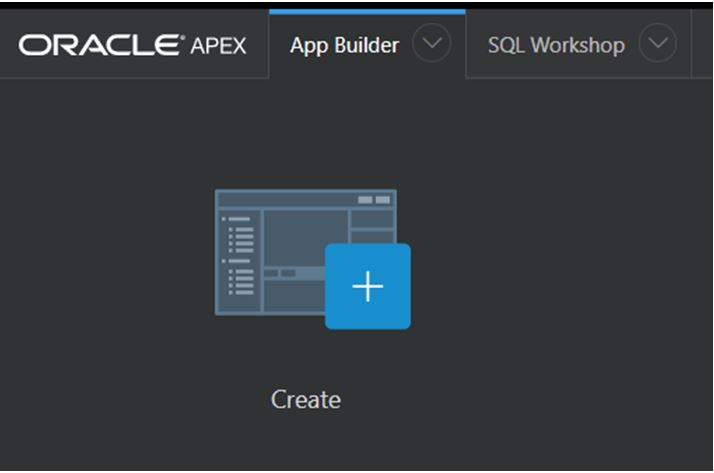
\includegraphics[scale=0.5]{section/gambar_bab1/3.JPG}
    \label{penanda}
\end{figure}
    \item request a workspace sudah dibuat dan submit
\begin{figure}[!htbp]
    \centering
    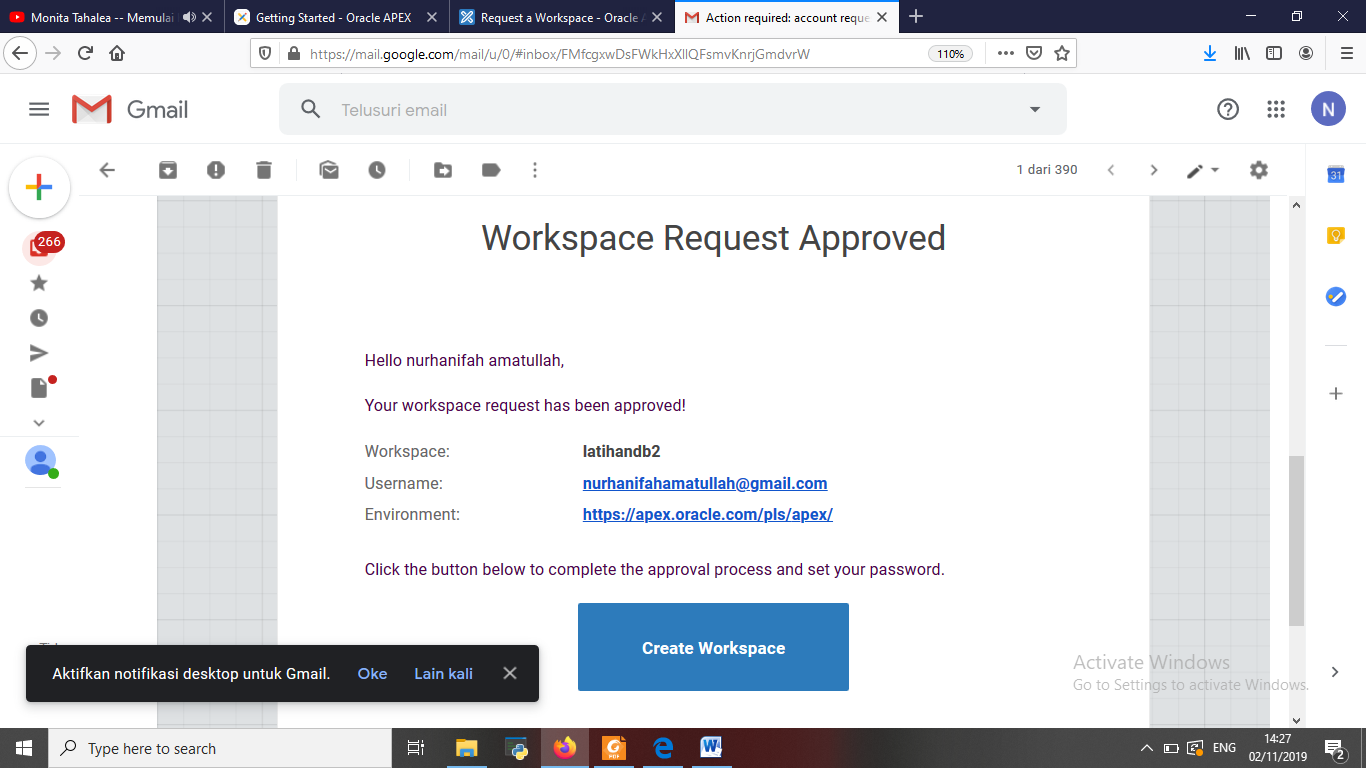
\includegraphics[scale=0.5]{section/gambar_bab1/6.JPG}
    \label{penanda}
\end{figure}   
\vspace{6cm}
    \item Lalu klik create workspace
\begin{figure}[!htbp]
    \centering
    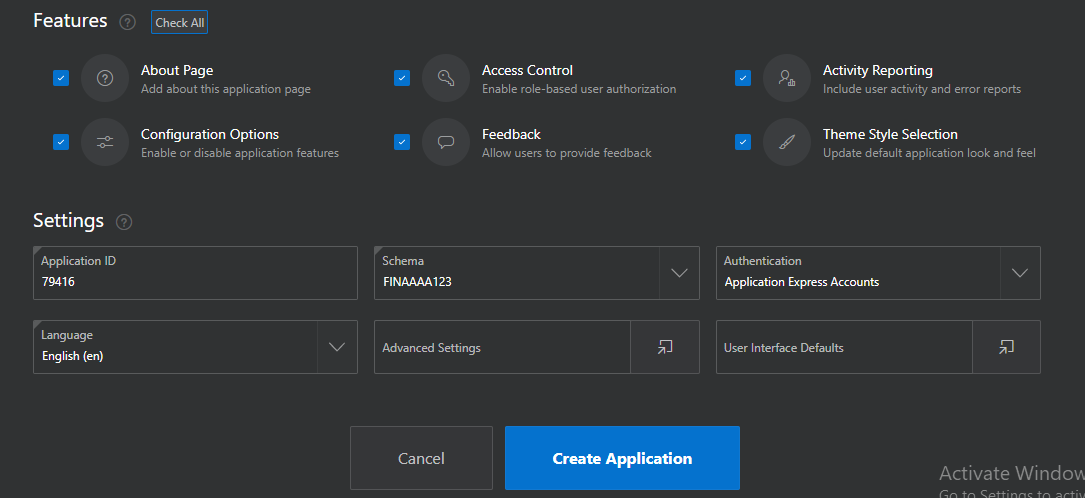
\includegraphics[scale=0.5]{section/gambar_bab1/8.JPG}
    \label{penanda}
\end{figure} 
\vspace{5cm}
    \item Lalu klik continiue to sign in screen
\begin{figure}[!htbp]
    \centering
    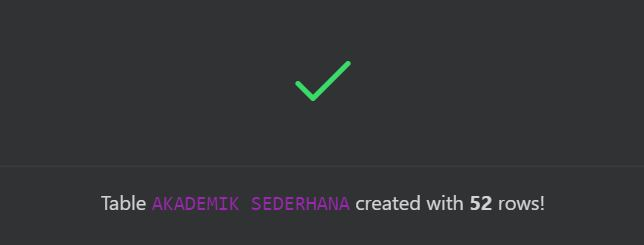
\includegraphics[scale=0.5]{section/gambar_bab1/9.JPG}
    \label{penanda}
\end{figure}
\vspace{6cm}
    \item Memasukkan ussername, password dan konfirmasi password. Lalu klik apply changes.
\vspace{3cm}
\begin{figure}[!htbp] 
    \centering
    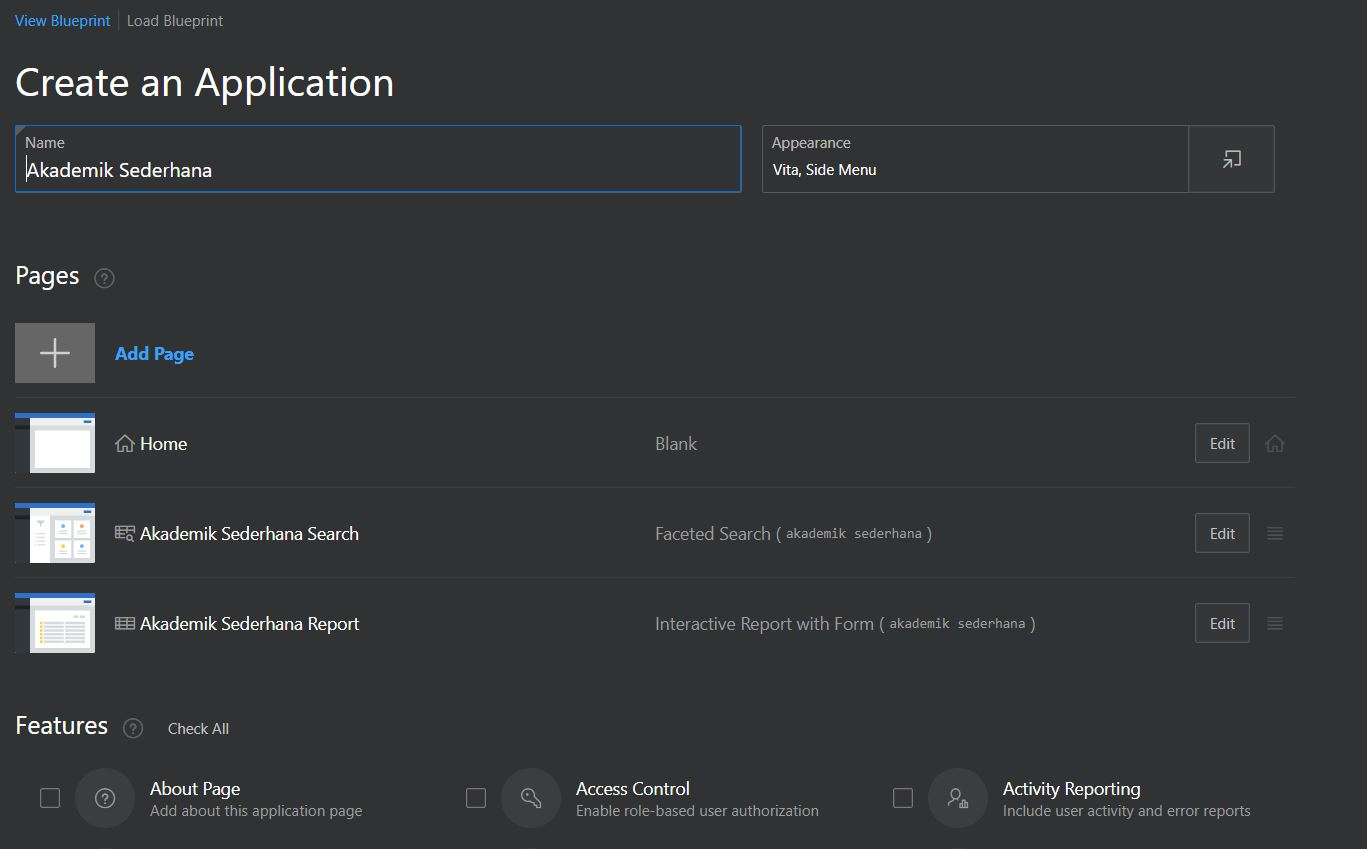
\includegraphics[scale=0.5]{section/gambar_bab1/10.JPG}
    \label{penanda}
\end{figure}
\vspace{16cm}
    \item Lalu klik App builder
\begin{figure}[!htbp]
    \centering
    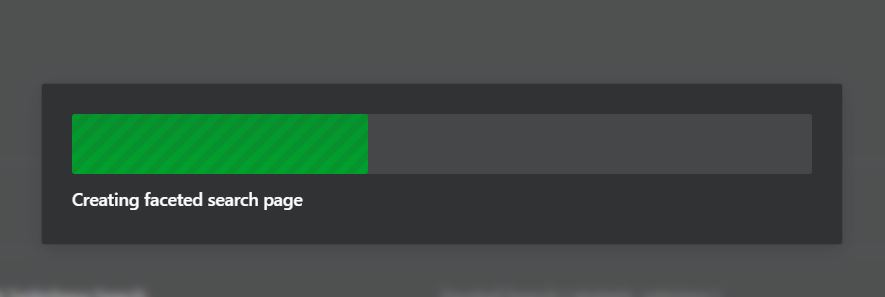
\includegraphics[scale=0.5]{section/gambar_bab1/11.JPG}
    \label{penanda}
\end{figure}
\vspace{16cm}
    \item Lalu klik create
\begin{figure}[!htbp]
    \centering
    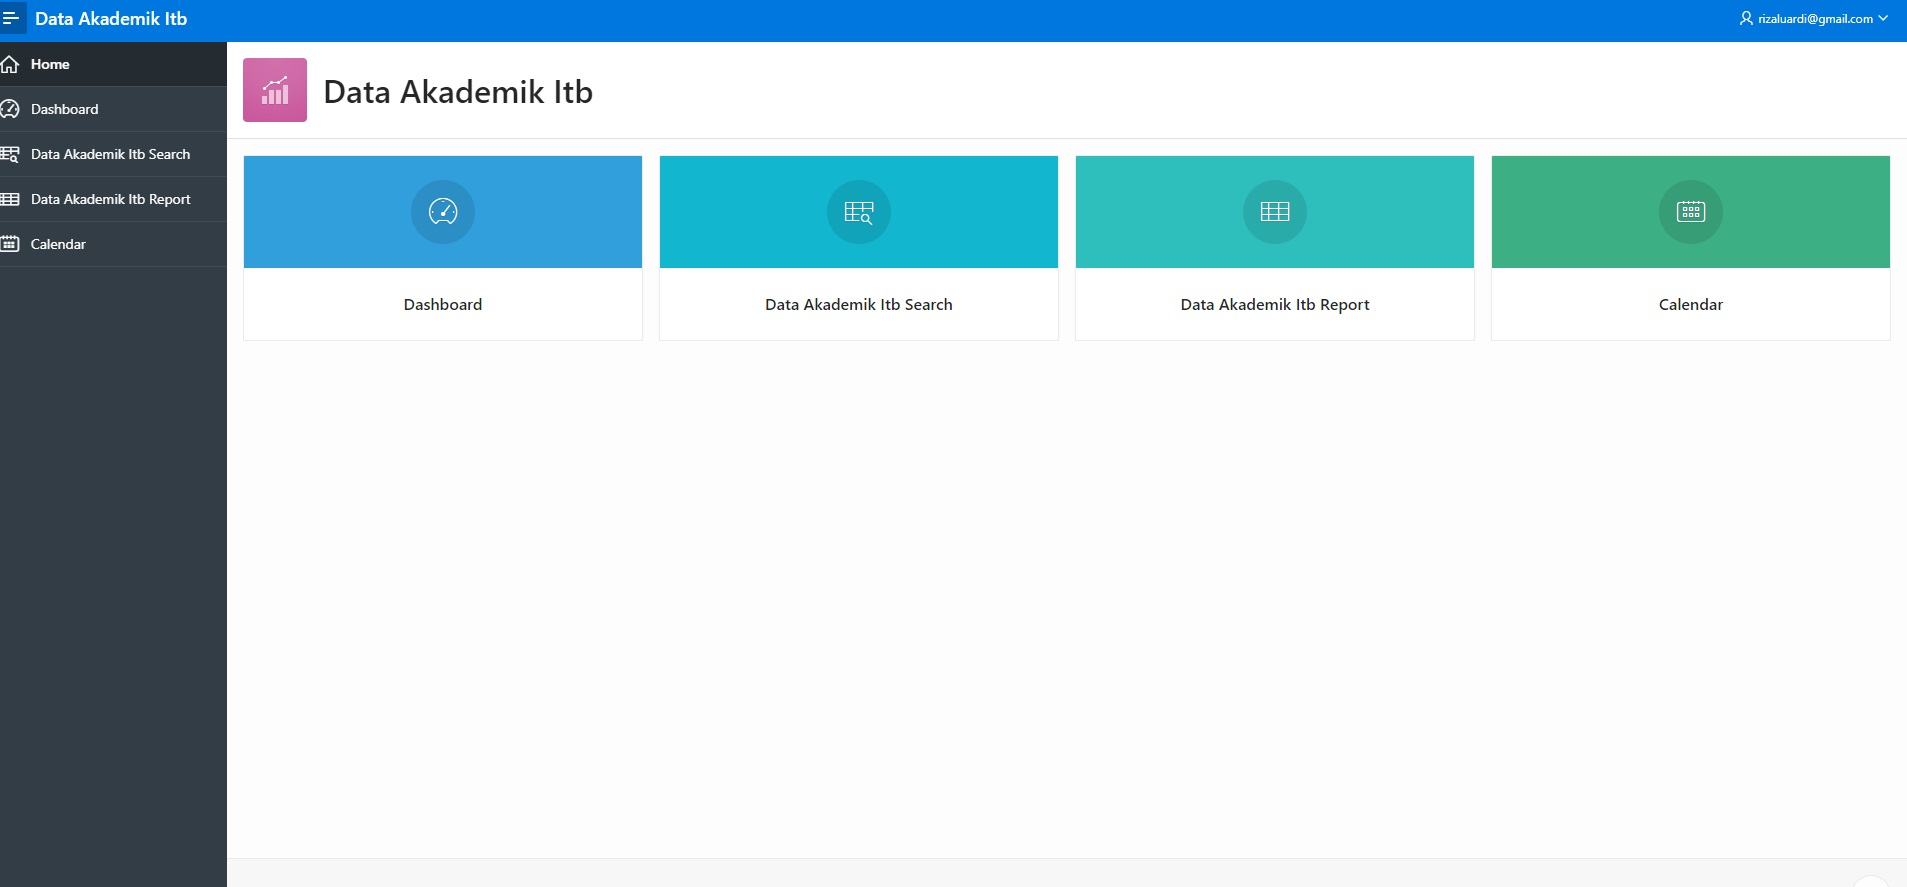
\includegraphics[scale=0.5]{section/gambar_bab1/12.JPG}
    \label{penanda}
\end{figure}
\vspace{16cm}
    \item Klik from a file
\begin{figure}[!htbp]
    \centering
    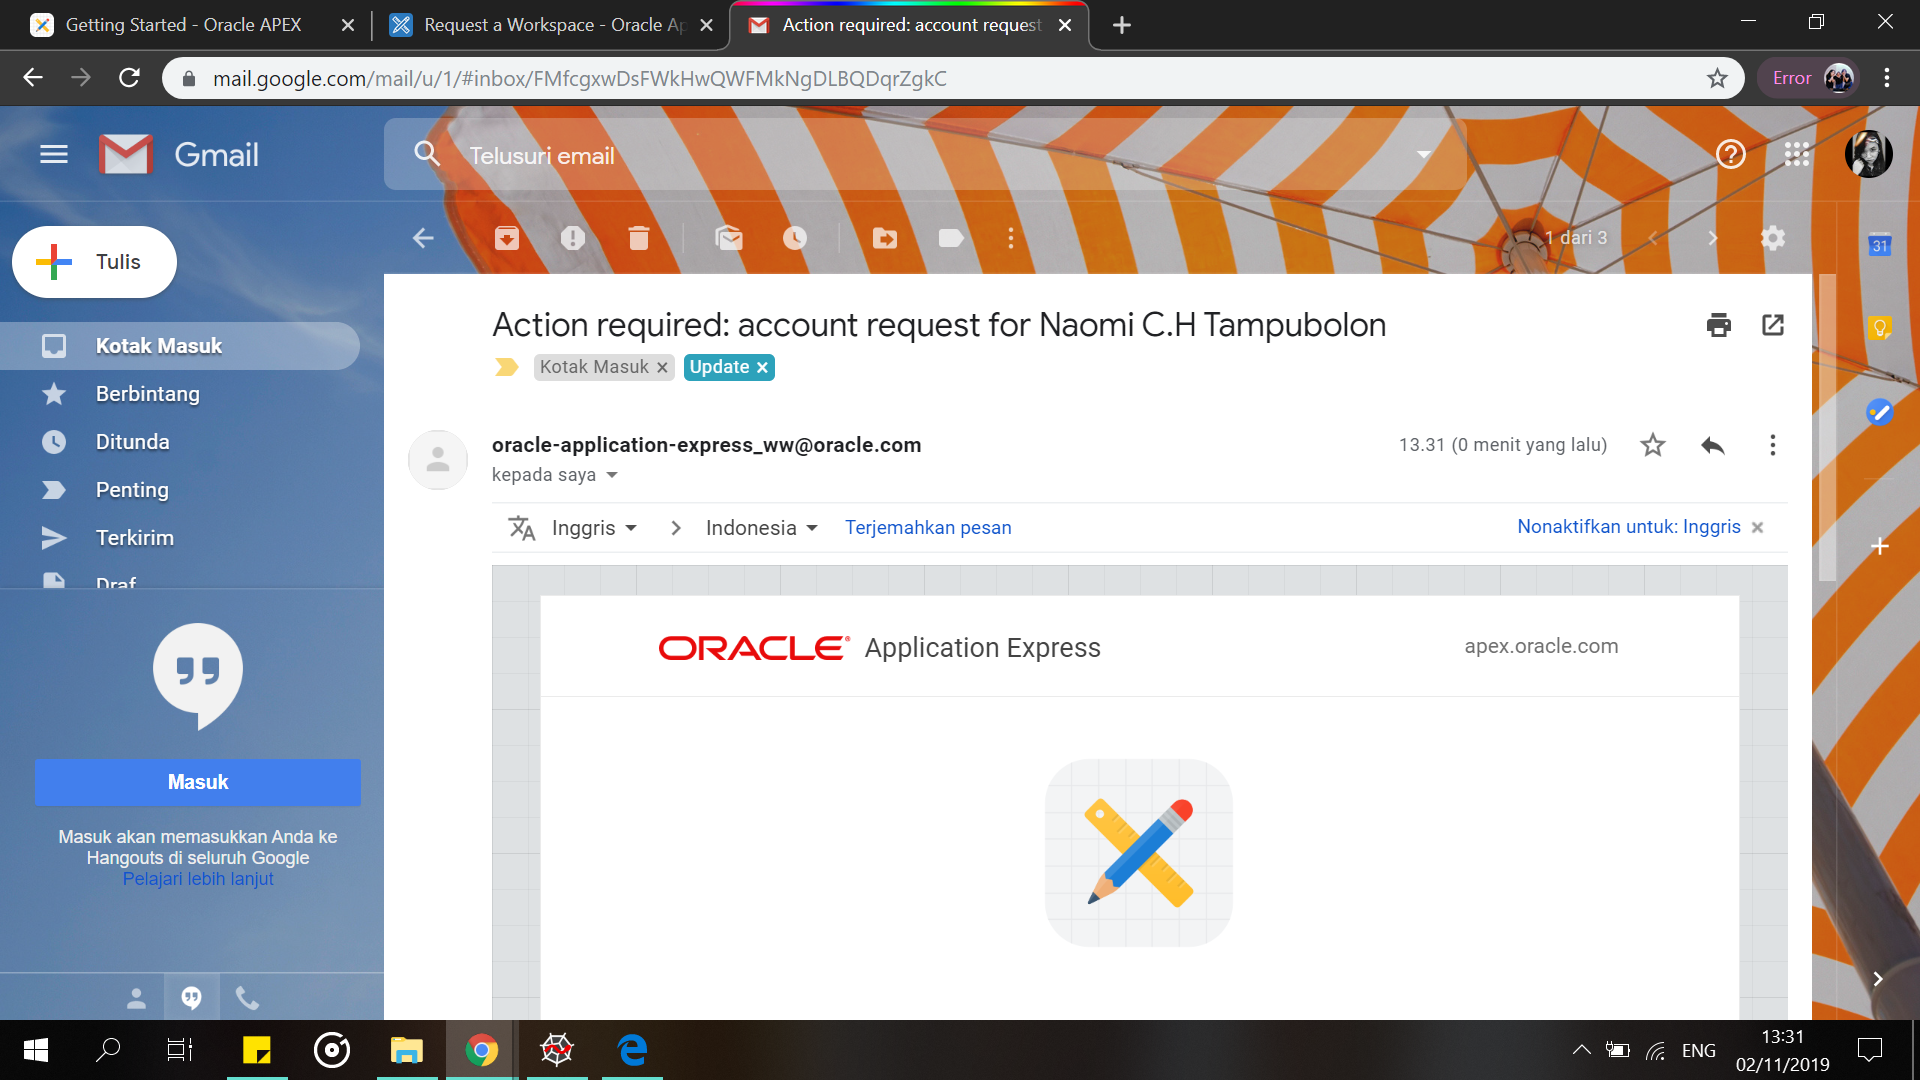
\includegraphics[scale=0.5]{section/gambar_bab1/13.JPG}
    \label{penanda}
\end{figure}
\vspace{16cm}
    \item Kemudian chose file, memilih file pada folder komputer/laptop
\begin{figure}[!htbp]
    \centering
    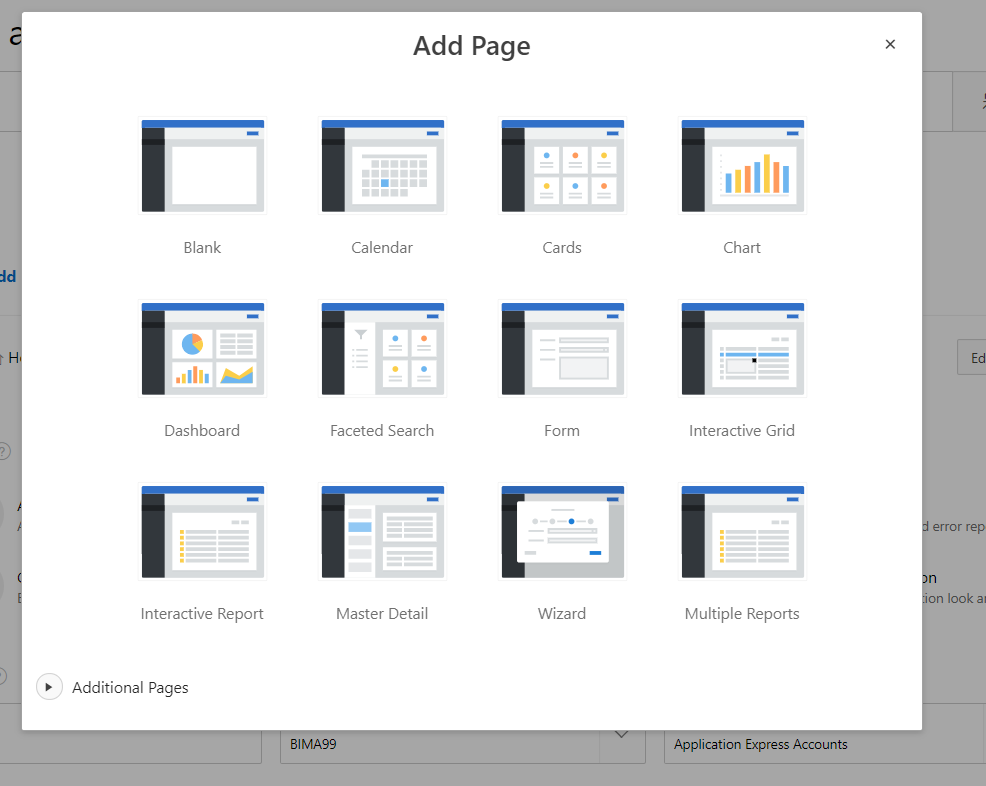
\includegraphics[scale=0.5]{section/gambar_bab1/14.JPG}
    \label{penanda}
\end{figure}
\vspace{16cm}
    \item membuat load data, jika sudah menyelesaikan menisi data tekan tombol load data pada pojok kanan layar
\begin{figure}[!htbp]
    \centering
    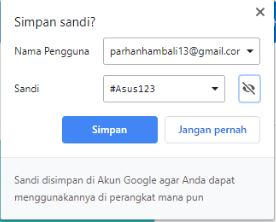
\includegraphics[scale=0.5]{section/gambar_bab1/15.JPG}
    \label{penanda}
\end{figure}
\vspace{16cm}
    \item Lalu klik tombol create application pada pojok kanan
\begin{figure}[!htbp]
    \centering
    
\includegraphics[scale=0.5]{section/gambar_bab1/16.JPG}
    \label{penanda}
\end{figure}
\vspace{16cm}
    \item Lalu klik lagi tombol create application pada pojok kanan
\begin{figure}[!htbp]
    \centering
    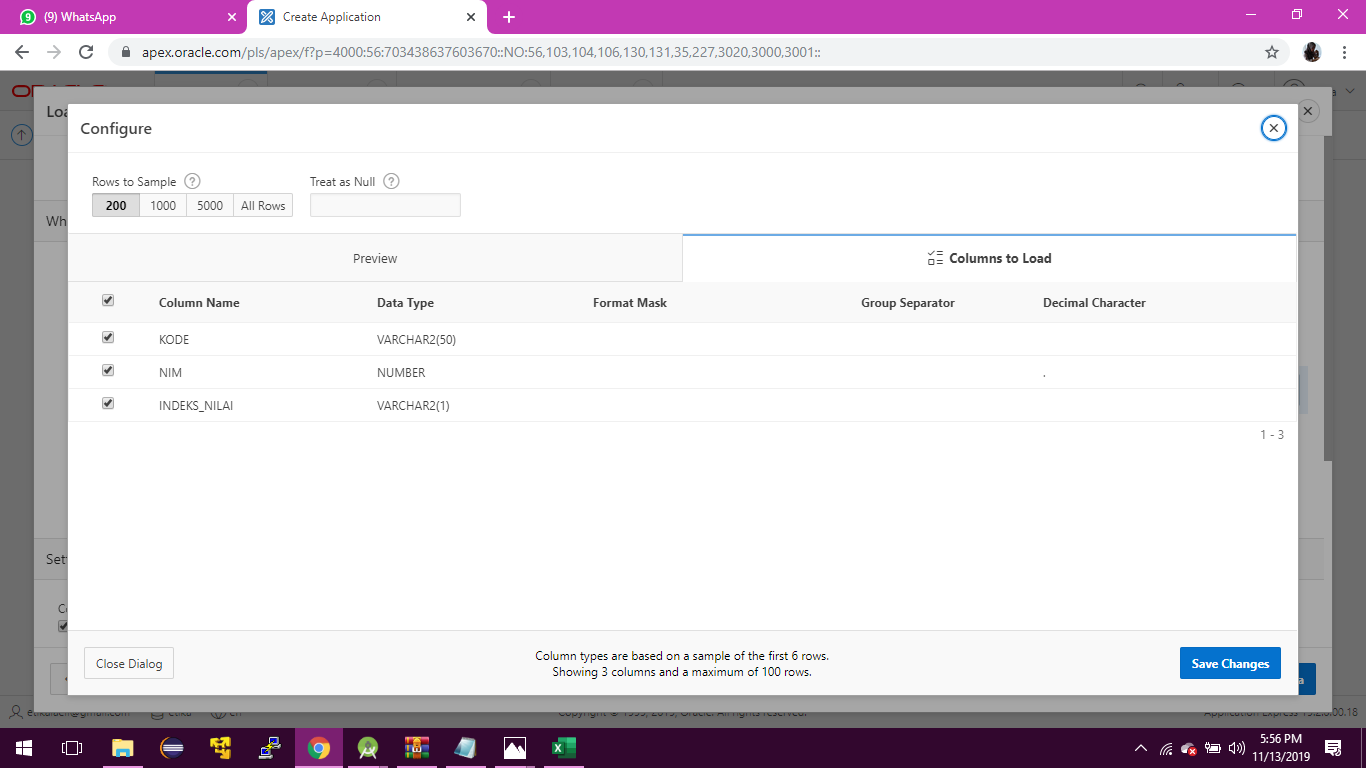
\includegraphics[scale=0.5]{section/gambar_bab1/17.JPG}
    \label{penanda}
\end{figure}
\vspace{16cm}
    \item Lalu Run application
\begin{figure}[!htbp]
    \centering
    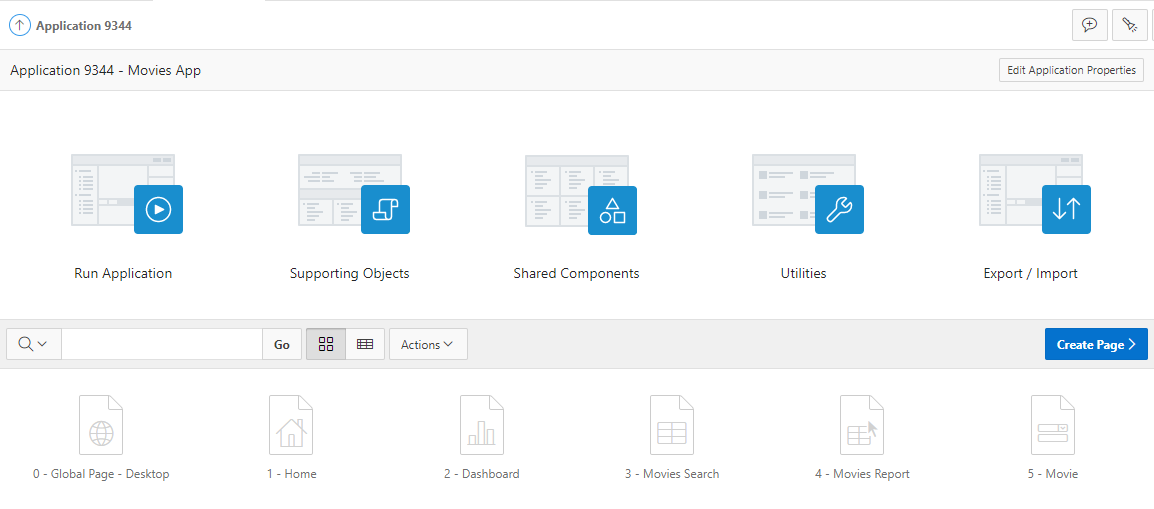
\includegraphics[scale=0.5]{section/gambar_bab1/18.JPG}
    \label{penanda}
\end{figure}
\vspace{10cm}
    \item Klik sign in
\begin{figure}[!htbp]
    \centering
    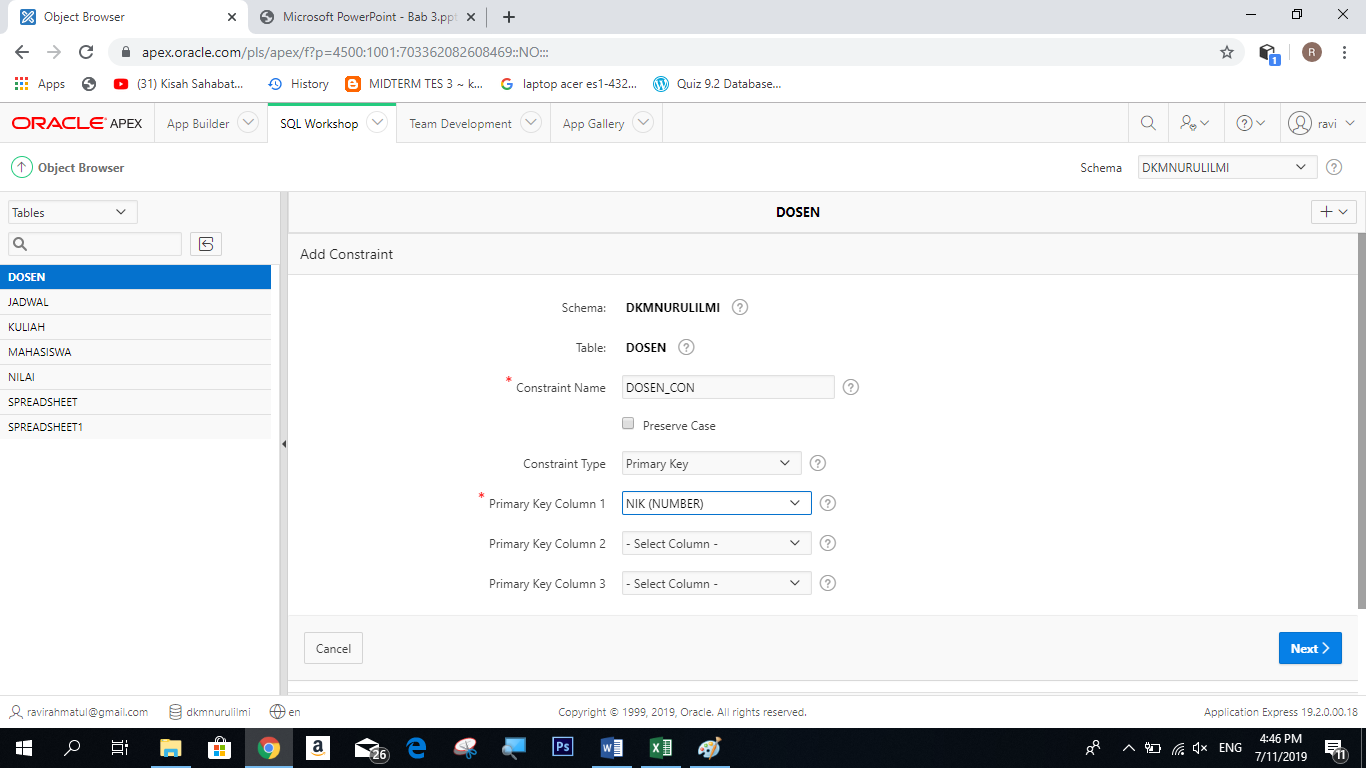
\includegraphics[scale=0.5]{section/gambar_bab1/19.JPG}
    \label{penanda}
\end{figure}
\vspace{10cm}
    \item selesai
\begin{figure}[!htbp]
    \centering
    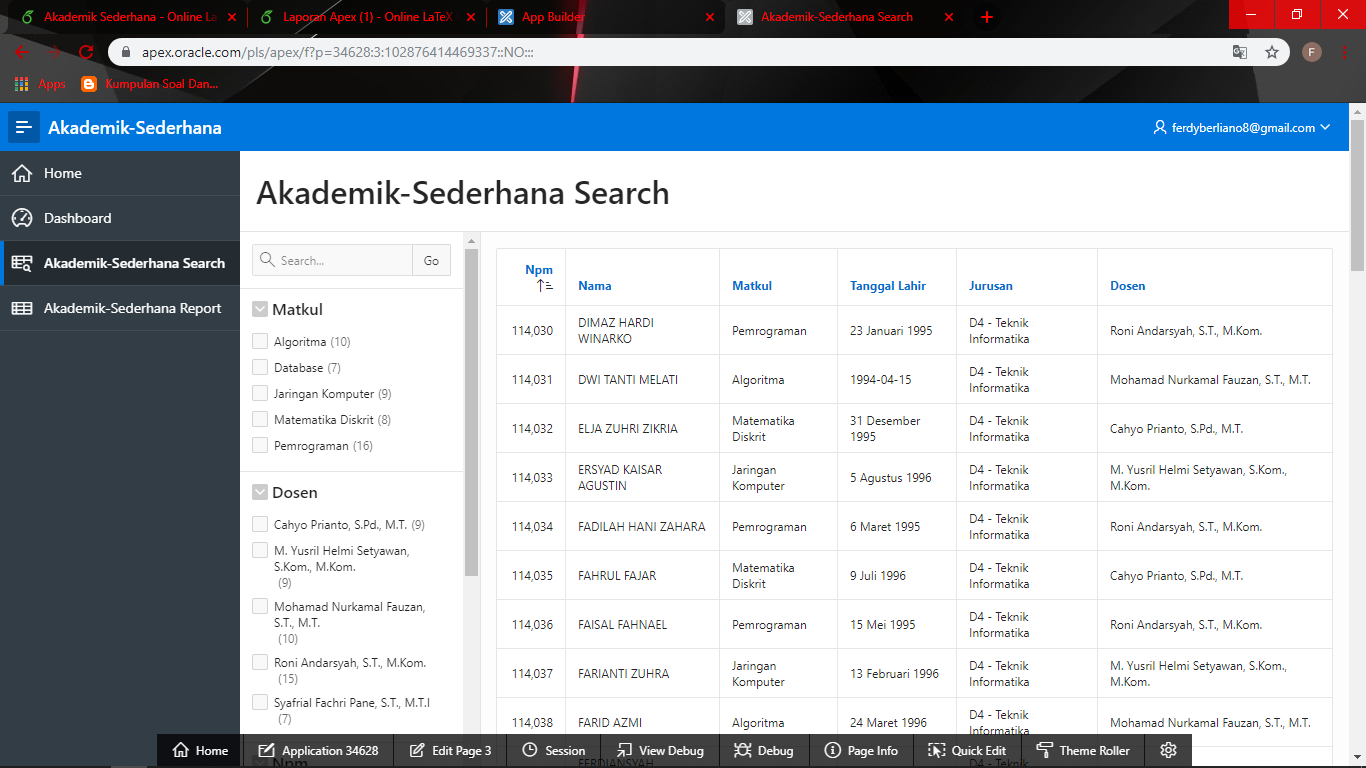
\includegraphics[scale=0.5]{section/gambar_bab1/20.JPG}
    \label{penanda}
\end{figure}
\end{enumerate}
link [https://apex.oracle.com/pls/apex/f?p=78916:LOGIN_DESKTOP:707736970168798:::::] 
username[nabillaahy@gmail.com] password[nabilla123]

\end{enumerate}